\documentclass{article}
\usepackage[a4paper, total={6in, 8in}]{geometry}
\usepackage[utf8]{inputenc}
\usepackage{graphicx}
\usepackage{todonotes}

\usepackage[pdftex,
            pdfauthor={Pablo Botas},
            pdftitle={Development report}]{hyperref}

\title{Development report}
% \date{}
\author{Pablo Botas}

\begin{document}
\maketitle

\todo[inline]{Is the CBCT read properly?}
\todo[inline]{Is the VF probing done at the appropriate position?}
\todo[inline]{How to fix the MHD/MHA output?}
\todo[inline]{Warping the endpoint and entrance point should not be done in parallel. When going further from the tramp center, a bigger angle should be applied!}


\section{Algorithm}

This is the implemented algorithm:

\begin{enumerate}
    \item Read patient data
    \item Assign a WEPL range to each spot using lut
    \item Raytrace each spot to get endpoint coordinates
    \begin{enumerate}
        \item Lose energy and WEPL voxel-by-voxel
        \item Stop if outside of CT, no WEPL or no energy
    \end{enumerate}
    \item Probe vector field at the endpoint positions
    \item Apply VF at endpoints
    \item Apply VF at starting points, neglecting the depth dimension with respect to the treatment plane (not individual spots)
    \item Raytrace each spot in the CBCT to get endpoint coordinates
    \item Compare with warped endpoint calculated at step 5 (along the same line, only depth difference)
    \item Assign energy shift for the depth difference: how to translate to energy?
\end{enumerate}

The adaptation is then:
\begin{itemize}
    \item XY inside the treatment plane as given by the VF for each spot
    \item Energy as given by the range difference at last step
\end{itemize}

\textbf{This effectively removes the layer organization in positions and energies.}

\section{Ray Tracing}

\begin{enumerate}
    \item A single ray is initialized per spot.
    \item The ray losses energy following the CSDA.
    \item When the ray has zero energy the endpoint is scored.
\end{enumerate}

\begin{figure}[h]
    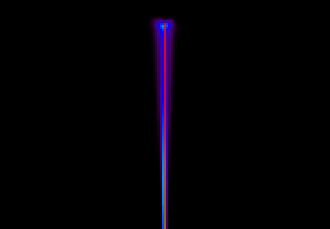
\includegraphics[width=0.49\textwidth]{beam.png}
    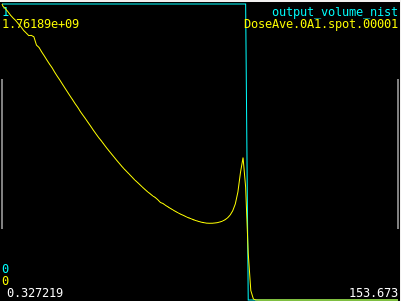
\includegraphics[width=0.49\textwidth]{profile.png}
    \caption{Beam with no $\sigma$ and $\epsilon$ in a patient (P15) and ray traced trajectory.}
\end{figure}

\section{Vector field probing}


\end{document}